% !TEX root = ../BScWIMEngl.tex

\chapter{Reinforcement Learning Algorithms}

\section{Introduction}

Dynamic Programming usually breaks down in the real world for two reasons:
\begin{enumerate}
    \item The transition probabilities and immediate rewards are not known or hard to calculate.
    \item The state and action space is too large to even compute one iteration of Dynamic Programming for every state-action tuple (e.g. possible positions and possible moves in every position in chess).
\end{enumerate}

This is where \emph{Reinforcement Learning} algorithms come in, which try to find solutions without having to sweep the entire state space. In this chapter based on \textcite{suttonReinforcementLearningIntroduction1998} (their second edition (\citeyear{suttonReinforcementLearningIntroduction2018a}) was used for statements which need to be up-to-date) we will examine advantages and disadvantages of various algorithms and discuss possible variations and extensions. In the next chapter we will attempt a proof of almost sure convergence of the basic algorithms introduced in this chapter, and illustrate their connection to stochastic approximation.

We separate their introduction and the convergence proofs, because -- while the guarantee of almost sure convergence is reassuring -- it is of little use for comparing various algorithms. Since one of the reasons for moving away from Dynamic Programming in the first place was, that we could not calculate the value function for the entire state space within a reasonable time frame, as the size of the state space is often too large for that. Therefore almost sure convergence should not be viewed as more than an entry requirement. For this reason most papers compare algorithms empirically on various example problems. And for some of the more complex algorithms convergence proofs simply do not exist yet. 

So since the theoretical convergence properties are usually only ever an afterthought, it is more natural to introduce the various algorithms heuristically, explaining what specific problems they try to address with examples.

\subsection{Naive Batch Learning}
Let us ignore the second problem of large state spaces for a moment and consider the case where we only have the first problem (\(p\) and \(r\) unknown). Then we can learn from a sample \(((X_t, A_t, Y_t, R_t), t\in\{0,\dots, T\})\) with
\[
	(Y_t,R_t)\sim \cP(\cdot \mid X_t, A_t)
\]
with the restriction \(Y_t=X_{t+1}\) if the sample is generated sequentially by a behaviour. But there is no reason not to allow this more general sample which might be useful in cases where you can jump around in the state space and try different transitions at will. 

We can then use this batch of transitions to calculate estimators \(\hat{p},\hat{r}\) for the state transitions and immediate rewards \(\hat{r}\). And use Dynamic Programming on these estimators.

\begin{algorithm}
	\caption{Naive Batch Learning Algorithm} \label{naive batch learning algorithm}
	\begin{enumerate}
		\item Generate the history \((X_t, A_t, Y_t, R_t, t\in\{0,\dots, T\})\)
		\begin{algorithmic}[1] 
			\For{ \((y,x,a)\in\cX\times\cX\times\cA \)} \Comment{initialize variables}
				\State rewards[\(x,a\)]\(\gets\)list() 
				\State stateTransitions[\(y\mid x,a\)]\(\gets\) 0
				\State totalTransitions[\(x,a\)]\(\gets\) 0
			\EndFor
			\For{\(t=0,\dots, T\)}
				\State rewards[\(X_t,A_t\)].append(\(R_{t+1}\))
				\State stateTransitions[\(Y_t\mid X_t,A_t\)]\(++\) \label{algo1: incr 1}
				\State totalTransitions[\(X_t,A_t\)]\(++\)\label{algo1: incr 2}
			\EndFor
			\For{\((x,a)\in\cX\times\cA\)}
				\State \(\hat{r}(x,a) \gets\) average(rewards[x,a])
				\For{\(y\in\cX\)}
					\State \(\hat{p}(y\mid x,a)\gets\) stateTransitions[\(y\mid x,a\)]\(/\)totalTransitions[\(x,a\)]\label{calculation of hat p}
				\EndFor
			\EndFor
		\end{algorithmic}
		\item Use Dynamic Programming on \(\hat{r}\), \(\hat{p}\) 
	\end{enumerate}
\end{algorithm}

If the batch was generated by an exploration policy we separated the \emph{exploration} from the later \emph{exploitation}. The methods which do that are often grouped under the term \emph{Batch Reinforcement Learning} or \emph{off-line} learning. 

This method works fine, if the state space is small and one can sample enough observations for every state and action in a reasonable timeframe.
But if our state space is too large for that, it is impractical to wait for this. 

%%%%%%%%%%%%%%%%%%%
\section{Monte Carlo}
%%%%%%%%%%%%%%%%%

One idea to tackle larger state spaces is, that it is often unnecessary to know the value function in every state.

To visualize this idea it is useful to imagine the state space to be a room the agent has to navigate. 

\[
\begin{tikzpicture}
	\foreach \x in {0,1,2,3,4}{
		\foreach \y in {0,1,2,3,4}{
			\draw (\x,\y) rectangle +(1,1);
		}
	}
	\node at (1.5,0.5){S};
	\node at (2.5,4.5) {\textcolor{gray}{\(\gamma^0\)}};
	\foreach \value in {2,3,4,5}{
		\tikzmath{
			int \power;
			\power=6-\value;
		}
		\node at (1.5, \value-0.5) {\textcolor{gray}{\(\gamma^\power\)}};
	}
	\node at (3.5, 4.5){G};
	

	\node at (8.5,2.5) {\parbox[t]{6cm}{The state space \(\cX\) are the tiles on the floor, the actions \(\cA\) are the adjacent tiles, where the next state is with probability one equal to the action, and the reward is 0 for every transition but the transition to the goal (G) where the reward is 1 and the game ends. The start state is S. The value of choosing a tile is indicated in grey on the tile for a selection of tiles.}};
\end{tikzpicture}
\]

It is often enough for the agent to know the action value function for the states on his path, without knowing the value of states in the corners. Since he can then follow these ``breadcrumbs'' to find the goal reliably again. And it will quickly stop walking in circles if it goes into the direction of the highest value next time. 

This idea is the basis for Monte Carlo algorithms. To make notation more brief we will introduce the algorithm to calculate the value function, the action value function will be analogous. Consider an episodic MDP and a behaviour \(\pi\), then
\[
	\sum_{t=0}^\infty\gamma^tR_{t+1}=\sum_{t=0}^T\gamma^tR_{t+1}
\]
is a bias free estimator for \(V^\pi(X_0)\) for episode length T. As the definition of \(V^\pi\) was
\[
	V^\pi(x)=\E\left[\sum_{t=0}^\infty\gamma^tR_{t+1} \;\middle|\; X_0=x \right], 
\]
and because of the Markov property,
\[
	\sum_{t=k}^T\gamma^tR_{t+1}
\]
is a bias free estimator for \(V^\pi(X_k)\). \emph{First-visit Monte Carlo} uses the return after the first visit of a state \(x\in\{X_1,\dots,X_t\}\) as an estimator for \(V^\pi(x)\).

\begin{algorithm}
	\caption{First-visit Monte Carlo}
	\begin{algorithmic}[1]
		\For{\(x\in\cX\)} \Comment{initializing}
			\State Returns\((x)\gets\) list()
			\State \(V^\pi(x)\gets 0\)
		\EndFor
		\While{true} (forever) \Comment{learning}
			\State Generate an episode \(((X_t,R_{t+1}), t\in\{0,\dots,T\})\) with behaviour \(\pi\)
			\For{\(x\in\{X_0,\dots,X_T\}\)}
				\State \(k\gets \min\{t \mid X_t=x\}\)
				\State Returns\((x)\).append(\(\sum_{t=k}^T\gamma^tR_{t+1}\))
				\State \(V^\pi(x)\gets\) average(Returns(x))
			\EndFor
		\EndWhile
	\end{algorithmic}
\end{algorithm}

Because of the strong law of large numbers, first-visit Monte Carlo algorithm causes the value function estimation \(\hat{V}^\pi(x)\) to converge with probability 1 to \(V^\pi(x)\), for every state \(x\in\cX\) which is visited with positive probability given a stationary behaviour \(\pi\) and starting distribution \(X_0\). This is due to the fact, that only one estimate for \(V^\pi(x)\) for an \(x\in\cX\) is used per episode, so all estimates are independent. And since the return after the first visit to \(x\) has the same distribution as the return conditional on the starting state being \(x\) conditional on the first visit to \(x\) existing (\ref{appx8}), these estimates are iid with expected value \(V^\pi(x)\).

\emph{Every-visit} Monte Carlo uses the Return after every visit of a state \(x\) to estimate \(V^\pi(x)\). Since this means that the tail of the rewards can be included in multiple returns, the returns are not independent from each other anymore which make proving convergence a little bit more difficult than simply applying the strong law of large numbers. Though every visit Monte Carlo will turn out to be a special case of TD(\(\lambda\)) (c.f. (\ref{batch TD(1) learning rate}), which lets us sketch some convergence proof ideas in Chapter \ref{stoch apprx}.

The same method can be applied to learn the action value function \(Q^\pi\). In this case we take the returns following a state \emph{and} action as estimators for \(Q^\pi\). But if the model is known and our problem is just a large state space calculating \(V^\pi\) is preferable, since \(|\cX|\le |\cX\times\cA|\) means that the first algorithm needs fewer observations to converge and \(Q^\pi\) can be calculated with \(V^\pi\) given \(r\) and \(p\).

\subsection{From \(\pi\) to \(\pi^*\)}
Let us assume exploring starts, i.e.
\[
	\Pr(X_0=x)>0 \qquad \forall x\in\cX,
\] 
for a moment. Then Monte Carlo converges whatever policy we select. Similar to policy iteration (Def. \ref{policy iteration}) we can then alternate between calculating \(Q^{\pi_n}\) and selecting \(\pi_{n+1}\) as a greedy policy with regard to \(Q^{\pi_n}\). This is referred to as generalized policy iteration (GPI). If we would wait for our Monte Carlo approximation of \(Q^{\pi_n}\) to converge, \(\pi_n\) would converge to \(\pi^*\) for the same reason as policy iteration converges. But remember we are doing Monte Carlo in the first place, because the state space is too large to wait for an evaluation of every state. Which means in practice algorithms alternate between choosing a greedy policy with regard to \({V^{\pi_n}}\) and generating an episode with policy \(\pi_n\), averaging the estimates from this episode with the estimates of \(V^{\pi_{n-1}}\). But since we have to assume
\[
	V^{\pi_{n-1}}\neq V^{\pi_n}
\] 
in general, using these old estimates is not bias free. It is easy to see that this procedure can only converge to \(\pi^*\) if it converges at all. Since there are only a finite number of deterministic stationary policies it would have to stay constant at some point, but for a constant policy Monte Carlo will converge, and then the policy can only stay constant if it is greedy with regards to its own value function, which forces it to be optimal (\ref{real improvement or optimal}). But it is still an open problem whether or not this alternating procedure converges at all \parencite[99]{suttonReinforcementLearningIntroduction2018a}.

If we remove the assumption of exploring starts, we still need to ensure that every state is visited with positive probability for MC to converge. This requires the policy to do the exploring. There are multiple approaches to exploration which we will discuss later (Section \ref{exploration}). We will discuss the most straightforward example here, under the assumption that we can calculate \(Q^{\pi_n}\) somehow.

\begin{definition}
	A stationary policy \(\pi\) is called 
	\begin{itemize}[font=\normalfont]
		\item \emph{soft}, if it fulfils 
		\[
			\pi(a\mid x)>0 \qquad\;\; \forall (x,a)\in\cX\times\cA,
		\]
		\item \emph{\(\vep\)-soft} for some \(1\ge \vep>0\), if it fulfils 
		\[
			\pi(a\mid x)>\frac{\vep}{|\cA_x|} \quad \forall (x,a)\in\cX\times\cA,
		\]
		\item \emph{\(\vep\)-greedy} with regard to Q, if it selects the greedy action w.r.t. Q with probability \((1-\vep)\) and a (uniform) random action with probability \(\vep\), i.e. \[\pi(a\mid x)=
			\begin{cases}
				(1-\vep)+ \frac{\vep}{|\cA_x|} & a \text{ is greedy\footnotemark[1]}\\
				\frac{\vep}{|\cA_x|} & a \text{ is not greedy}.
			\end{cases}
		\]
	\end{itemize}\footnotetext[1]{w.l.o.g. only one greedy action, otherwise pick one or mix}
	Note that an \(\vep\)-greedy policy is \(\vep\)-soft.

	An \(\vep\)-soft policy \(\pi^*\) is called \emph{\(\vep\)-soft optimal} if 
	\[
		V^{\pi^*}(x)=\sup_{\pi\; \vep\text{-soft}}(x) V^\pi \eqqcolon \tilde{V}^*(x).
	\]
\end{definition}

\begin{prop}
	Generalized policy iteration with \(\vep\)-greedy policies converges to an \(\vep\)-soft optimal policy
\end{prop}
\begin{proof}
	% Let \(\pi_{n+1}\) be \(\vep\)-greedy with regard to \(Q^{\pi_n}\). Since \(\pi_n\) is an \(\vep\)-soft policy we know that
	% \[
	% 	\pi_n(a\mid x) -\frac{\vep}{|\cA_x|} \ge 0
	% \]
	% which together with the equality
	% \[
	% 	\sum_{a\in\cA_x}\frac{\pi_n(a\mid x) -\frac{\vep}{|\cA_x|}}{1-\vep} 
	% 	= \frac{\left(\sum_{a\in\cA_x}\pi_n(a\mid x)\right)- \vep}{1-\vep}
	% 	= 1
	% \]
	% implies the inequality (\ref{weighted sum}). Since the maximum is larger than the weighted average.
	% \begin{align}
	% 	&T^{\pi_{n+1}}V^{\pi_n}(x)=Q^{\pi_n}(x,\pi_{n+1}(x))
	% 	=\sum_{a\in\cA_x} \pi_{n+1}(a\mid x) Q^{\pi_n}(x,a)
	% 	\nonumber\\
	% 	&\lxeq{\vep\text{-greedy}}\frac{\vep}{|\cA_x|}\sum_{a\in\cA_x}Q^{\pi_n}(x,a)
	% 	+(1-\vep)\max_{a\in\cA_x} Q^{\pi_n}(x,a)
	% 	\nonumber\\
	% 	&\ge\frac{\vep}{|\cA_x|}\sum_{a\in\cA_x}Q^{\pi_n}(x,a) 
	% 	+(1-\vep)\sum_{a\in\cA_x}
	% 	\frac{\pi_n(a\mid x) -\frac{\vep}{|\cA_x|}}{1-\vep}Q^{\pi_n}(x,a)  
	% 	\label{weighted sum}\\
	% 	&=\frac{\vep}{|\cA_x|}\sum_{a\in\cA_x}Q^{\pi_n}(x,a) 
	% 	-\frac{\vep}{|\cA_x|}\sum_{a\in\cA_x}Q^{\pi_n}(x,a)
	% 	+\sum_{a\in\cA_x}\pi_n(a\mid x)Q^{\pi_n}(x,a)
	% 	\nonumber\\
	% 	&=V^{\pi_n}(x)\nonumber
	% \end{align}
	% This implies \(V^{\pi_{n+1}}\ge V^{\pi_n} \). 
	To use the same argument as with standard policy iteration (\ref{real improvement or optimal}), we would need
	\[
		T^*(V^{\pi_n})=T^{\pi_{n+1}}(V^{\pi_n}).
	\]
	But this is not true. To circumvent this problem we ``move the requirement of \(\vep\)-softness into the environment''. I.e. we define an MDP \(\tilde{M}\) where
	\[
		\tilde{\cP}(\cdot \mid x,a) \coloneqq (1-\vep) \cP(\cdot \mid x,a) 
		+ \frac{\vep}{|\cA_x|}\sum_{b\in\cA_x} \cP(\cdot \mid x,b).
	\]
	This means, that with probability \(\vep\), the transition kernel will ignore the selected action and behave as if an uniformly random action was chosen.	
	
	We can transform \(\vep\)-soft policies \(\pi\) from the old MDP to stationary policies \(\tilde{\pi}\) of \(\tilde{M}\) with a mapping \(f\), where
	\[
		f(\pi)(a\mid x)=\tilde{\pi}(a\mid x)\coloneqq \frac{\pi(a\mid x)-\frac{\vep}{|\cA_x|}}{1-\vep}\ge 0.
	\]
	And for every stationary policy \(\tilde{\pi}\) of \(\tilde{M}\) we can define the \(\vep\)-soft policy \(\pi\) by
	\[
		\pi(a\mid x)\coloneqq (1-\vep)\tilde{\pi}(a\mid x) + \frac{\vep}{|\cA_x|},
	\]
	which is the inverse mapping. Therefore \(f\) is a bijection between the \(\vep\)-soft policies in the old MDP and all stationary policies in the new MDP. We now show, that the Value functions \(V^\pi\) stay invariant with regard to this mapping. 
	First note:
	\begin{align*}
		\tilde{p}(y\mid x,a)
		&=\tilde{\cP}(\{y\}\times \R\mid x,a)\\
		&=(1-\vep)p(y\mid x,a)+\frac{\vep}{|\cA_x|}\sum_{b\in\cA_x}p(y\mid x,b)
	\end{align*}
	And together with \(q(B\mid x,a)\coloneqq \cP(\cX\times B \mid x,a)\), the complementary marginal distribution which hast the same property, we can show:
	\begin{align*}
		\tilde{r}(x,a)&=\int t\ d\tilde{q}(t \mid x,a)=\int t\ 
		d\left((1-\vep)q(\cdot\mid x,a) + \frac{\vep}{|\cA_x|}\sum_{b\in\cA_x}q(\cdot\mid x,b)\right)(t) \\
		&=(1-\vep)\int t\ dq(t\mid x,a) 
		+ \frac{\vep}{|\cA_x|}\sum_{b\in\cA_x} \int t\ dq(t\mid x,a)\\
		&=(1-\vep)r(x,a) + \frac{\vep}{|\cA_x|}\sum_{b\in\cA_x}r(x,b)
	\end{align*}
	Therefore we know:
	\begin{align*}
		&\sum_{a\in\cA_x}\tilde{\pi}(a\mid x)\tilde{r}(x,a)\\
		&=\sum_{a\in\cA_x} \left(\frac{\pi(a\mid x)-\frac{\vep}{|\cA_x|}}{1-\vep} \right)
		\left((1-\vep)r(x,a) + \frac{\vep}{|\cA_x|}\sum_{b\in\cA_x}r(x,b)\right)\\
		&=\sum_{a\in\cA_x}\left(\pi(a\mid x)-\frac{\vep}{|\cA_x|}\right)r(x,a) 
		+ \frac{\vep}{|\cA_x|}\sum_{b\in\cA_x}r(x,b) 
		\underbracket[0.7pt]{\sum_{a\in\cA_x}\frac{\pi(a\mid x)-\frac{\vep}{|\cA_x|}}{1-\vep}}_{
			=1
		}\\
		&=\sum_{a\in\cA_x}\pi(a\mid x)r(x,a)
	\end{align*}
	And similarly:
	\begin{align*}
		&\Pr^{\tilde{\pi}}(\tilde{X}_1=y\mid \tilde{X}_0=x) 
		=\sum_{a\in\cA_x}\tilde{\pi}(a\mid x)\tilde{p}(y\mid x,a)\\
		&=\sum_{a\in\cA_x}\left(\frac{\pi(a\mid x)-\frac{\vep}{|\cA_x|}}{1-\vep} \right)
		\left((1-\vep)p(y\mid x,a)+\frac{\vep}{|\cA_x|}\sum_{b\in\cA_x}p(y\mid x,b)\right)\\
		&=\dotsc = \sum_{a\in\cA_x} \pi(a\mid x)p(y\mid x,a) =\Pr^\pi(X_1=y\mid X_0=x)
	\end{align*}
	The last two equations imply together:
	\begin{align*}
		\tilde{T}^{\tilde{\pi}}V^\pi(x)&=\sum_{a\in\cA_x}\tilde{\pi}(a\mid x)\tilde{r}(x,a) 
		+ \gamma \sum_{y\in\cX}\Pr^{\tilde{\pi}}(\tilde{X}_1=y\mid X_0=x)V^\pi(y)\\
		&=\sum_{a\in\cA_x}\pi(a\mid x)r(x,a) + \gamma \sum_{y\in\cX}\Pr^\pi(X_1=y\mid X_0=x)V^\pi(y)\\
		&=T^\pi V^\pi(x)=V^\pi(x)
	\end{align*}
	And since the fixpoint is unique it follows that
	\[
		V^{\tilde{\pi}}=V^\pi.
	\]
	And as f is bijective, this implies
	\[
		\sup_{\tilde{\pi}\in \tilde{\Pi}_S}V^{\tilde{\pi}}(x)=\sup_{\pi\ \vep\text{-soft}} V^\pi(x),
	\]
	as well as:
	\begin{align*}
		Q^{\tilde{\pi}}(x,a)&=\tilde{r}(x,a)+\gamma \sum_{y\in\cX} \tilde{p}(y\mid x,a) V^\pi(y)\\
		&=\begin{aligned}[t]
			&(1-\vep)\left(r(x,a)+\gamma \sum_{y\in\cX}p(y\mid x,a) V^\pi(y) \right)\\
			&\qquad + \frac{\vep}{|\cA_x|}\sum_{b\in\cA_x}\left(r(x,b)+\gamma \sum_{y\in\cX}p(y\mid x,b) \right)
		\end{aligned}\\
		&=(1-\vep)Q^\pi(x,a)
		+ \frac{\vep}{|\cA_x|}\sum_{b\in\cA_x}\left(r(x,b)+\gamma \sum_{y\in\cX}p(y\mid x,b) \right)
	\end{align*}
	Which implies that
	\[
		\arg\max_{a\in\cA_x} Q^{\tilde{\pi}}(x,a)=\arg\max_{a\in\cA_x} Q^\pi(x,a).
	\]
	Therefore greedy with regard to \(Q^\pi\) and \(Q^{\tilde{\pi}}\) is the same. Let \(\pi_n\) be an \(\vep\)-soft policy, and let \(\pi_{n+1}\) be \(\vep\)-greedy with regard to 
	\(Q^{\pi_n}\). Then \(\tilde{\pi}_{n+1}\coloneqq f(\pi_{n+1})\) is greedy w.r.t. 
	\(Q^{\tilde{\pi}_n}\):
	\begin{align*}
		\tilde{\pi}_{n+1}(a\mid x)&=f(\pi_{n+1})(a\mid x)
		=\frac{\pi(a\mid x)-\frac{\vep}{|\cA_x|}}{1-\vep}\\
		&=\begin{cases}
			\frac{\left((1-\vep) + \frac{\vep}{|\cA_x|}\right) -\frac{\vep}{|\cA_x|}}{1-\vep}=1 & a \text{ is greedy}\\
			\frac{\frac{\vep}{|\cA_x|}- \frac{\vep}{|\cA_x|}}{1-\vep}=0 & a \text{ is not greedy}
		\end{cases}
	\end{align*}
	Since we proved policy iteration converges for greedy policies, this finishes our proof:
	\[
		\sup_{\pi\ \vep\text{-soft}} V^\pi(x)
		=\sup_{\tilde{\pi}\in \tilde{\Pi}_S}V^{\tilde{\pi}}(x)
		=\lim_{n\to\infty} V^{\tilde{\pi}_n}(x)
		=\lim_{n\to\infty} V^{\pi_n}(x)
		\qedhere
	\]
\end{proof}


\subsection{Shortcomings of Monte Carlo}
\citeauthor{suttonReinforcementLearningIntroduction1998} provide a very instructive example for the weakness of Monte Carlo. Recall that Monte Carlo tries to estimate \(V^\pi\). So the example assumes a given behaviour and tries to evaluate the value of a situation.

\begin{example}[Driving Home]\label{driving home}
	Let us assume that John Doe works in city A, and drives to his home in city B after work, every day. Since he wants to get home as quickly as possible, the value of the state is inversely proportional to the time it will take him from a certain position home. This means that estimating the value of a certain state is equivalent to estimating the time left to drive. The longer John drives this route, the better he will get, at estimating the time it will take him to drive certain sections of the road. If there is a delay in an earlier section he has a good estimate for the remaining time, once he clears the obstruction. Now imagine he is driving home from a doctors appointment from city A. As soon as he enters the highway to city B, he is able to use his experience driving this route to estimate the remaining time quite precisely.

	The Monte Carlo algorithm on the other hand \emph{never} uses existing value estimations to estimate the value of a different state. If John Doe uses Monte Carlo estimates to guess the remaining time from the doctor, the accuracy of his estimates will only ever increase with the times he actually starts driving from the doctor's office. 
\end{example}

Since Monte Carlo has more possible "starting points", or generally earlier points in the chain, in case of estimating \(Q^\pi\), it is worse in this case. An extreme example would be two actions in the same state, which have the same effect. Even though Monte Carlo might have a good estimate of the value of the first action it will start completely anew for the second action. 

\section{Temporal Difference Learning TD}
Temporal Difference learning (TD), first proposed by \textcite{suttonLearningPredictMethods1988}, addresses this weakness of Monte Carlo algorithms. 

For a sequence \((X_t,A_t,R_{t+1}, {t\in\N_0})\) generated by a stationary behaviour \(\pi\), we know: 
\begin{align}
	&\E^\pi[R_{t+1}+\gamma V(X_{t+1})\mid X_t=x] 
	\nonumber\\
	&=\E^\pi[r(x,A_0)\mid X_0=x]+\gamma\sum_{y\in\cX}\Pr^\pi(X_1=y\mid X_0=x)V(y) 
	\nonumber\\
	&= T^\pi V(x) \label{estimates T^pi V}
\end{align}
The random variable \(R_{t+1}+\gamma V(X_{t+1})\) is therefore a bias free estimator for \(T^\pi V (X_t)\). But because of its variance we can not simply update \(V(X_t)\). Instead TD moves the estimate into the direction of this observation. To get an intuition for why this makes sense consider this example.
\begin{example}[Unwinding the Arithmetic Mean]\label{unwinding the mean}
	Let \(X_i\) be independent identically distributed (iid) random variables, then the arithmetic means is:
	\begin{align*}
		\widebar{X}_n&=\mfrac{1}{n}\sum_{i=1}^n X_i 
		= \mfrac{n-1}{n}\mfrac{1}{n-1}\sum_{i=1}^{n-1}X_i +\mfrac{1}{n}X_n\\
		&=\left(1-\mfrac{1}{n}\right)\widebar{X}_{n-1}+\mfrac{1}{n}X_n \\
		&= \widebar{X}_{n-1} + \underbracket[0.7pt][1.3ex]{\frac{1}{n}}_{\text{\clap{``learning rate''}}}\underbracket[0.7pt][0.4ex]{(X_n - \widebar{X}_{n-1})}_{\text{``direction''}}
	\end{align*}
\end{example}

But Temporal Difference Learning tries to do Dynamic Programming (i.e. replacing \(V\) with \(T^\pi V\), which would require a learning rate of \(1\)) at the same time as trying to reduce the error of the estimate of \(T^\pi V\), where the learning rate should be something like \(1/n\). The smaller the learning rate, the more of the old estimate we retain. This has the disadvantage, that old estimates are (in a way) previous steps in dynamic programming, which are further away from \(V^\pi\). Larger learning rates on the other hand retain more of the variance of the latest random variable in the estimator. So one might for example want to have larger steps at the beginning until the dynamic programming part converges, and then start to focus more on the variance reduction part. This implies that a wider range of learning rates might be sensible. More on that in the third chapter. We therefore define 
\begin{align}\label{TD learning}
	V_{n+1}(x) \coloneqq
	\begin{cases}
		V_n(x)+\alpha_n[R_{n+1}+\gamma V_n(X_{n+1}) - V_n(x)] & x=X_n\\
		V_n(x) & x\neq X_n,
	\end{cases}
\end{align}
where \(\alpha_n\) is called the \emph{learning rate}. As one might want to increase the learning rates for rarely visited areas of the MDP, and decrease it for well known parts, it makes sense to allow it to be a function of the history \(((X_t, A_t, R_{t+1}), t\in\{0,\dots, n\})\) and thus allow it to be a random variable. We will omit this possible dependency for now and reconsider it in Chapter \ref{stoch apprx}.

For a deterministic stationary behaviour \(\pi\), we can show the analogue 
\begin{align*}
	&\E^\pi[R_{t+1}+\gamma Q(X_{t+1}, A_{t+1})\mid X_t=x, A_t=a]\\
	&=r(x,a) +\gamma \sum_{y\in\cX}p(y\mid x,a)Q(y,\pi(y))\\
	&= T^\pi Q(x,a).
\end{align*}
Note that we could easily extend this to all stationary policies (c.f. \ref{expand Q^pi}, \ref{T^pi unique}), by defining
\[
	T^\pi Q(x,a)\coloneqq r(x,a) +\gamma \smashoperator{\sum_{(y,b)\in\cX\times\cA}}\Pr^\pi[X_{t+1}=y,A_{t+1}=b\mid X_t=x,A_t=a]Q(y,b).
\]

To distinguish the TD algorithm, which calculates \(Q\) from the one which calculates \(V\), \citeauthor{suttonReinforcementLearningIntroduction1998} call the first one \emph{Sarsa}. The name stems from the tuple \((S_t, A_t,R_{t+1},S_{t+1},A_{t+1})\), as \(S_t\) is their notation for the state. 

\begin{algorithm}
	\caption{On-line Sarsa \parencite{suttonReinforcementLearningIntroduction1998}}
	Assume there is a mapping \(\Psi\), assigning an action value function Q a policy \(\pi\) (for example mapping Q on an \(\vep\)-greedy policy w.r.t. Q).
	\begin{algorithmic}[1]
		\State initialize Q(x,a)
		\While{True} (for every episode)
			\State initialize \(x\) as a realization of \(X_0\)
			\State choose \(a\) according to \(\Psi(Q)(\cdot \mid x)\)
			\Repeat(for each step \(n\) of the episode)
				\State do \(a\), observe reward \(R\) and next state \(y\)
				\State choose \(b\) according to \(\Psi(Q)(\cdot \mid y)\)
				\State \(Q(x,a)\gets Q(x,a) + \alpha_n [R+\gamma Q(y,b) -Q(x,a) ]\)
				\State \(x\gets y\); \(a\gets b \)
			\Until{x is terminal}
		\EndWhile
	\end{algorithmic}
	Where \(\alpha_n\) is the learning rate.
\end{algorithm}

Similar to the Monte Carlo algorithm, we use generalized policy iteration to approach \(\pi^*\). But since we do not need to wait for an episode to finish to create new estimates, we can alternate even more quickly between calculating \(Q^{\pi_n}\) and selecting \(\pi_{n+1}\). The most extreme form is now updating the policy before every transition in every time step. This is what is called \emph{on-line} learning in contrast to the \emph{off-line} mentioned in the introduction. 

Batch Reinforcement Learning is often used synonymously with off-line learning. But as batch learning algorithms were designed to utilize the information of the existing batch as efficiently as possible, there were some attempts to modify them in order to provide intermediate results to advise action selection, transforming them into on-line algorithms. \textcite{langeBatchReinforcementLearning2012} suggest to refer to these algorithms as \emph{growing batch reinforcement learning}. We will discuss an example in Section \ref{growing batch learning}, after explaining the need for it. 

\subsection{Shortcomings of TD} \label{shortcomings TD}
In a way TD is the opposite of Monte Carlo. While Monte Carlo did not use existing estimates of the value function, TD \emph{only} uses existing estimates. This can cause problems as well.

\begin{wrapfigure}{r}{5.5cm}
	\begin{centering}
		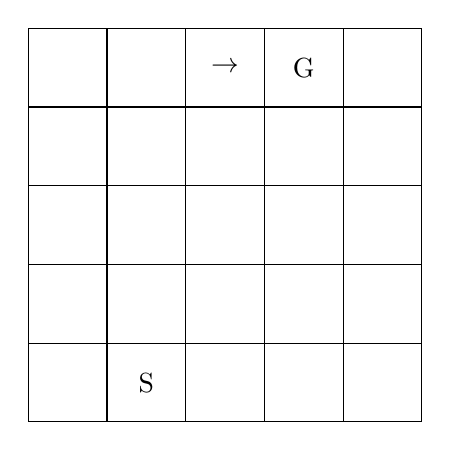
\begin{tikzpicture}
			\foreach \x in {0,1,2,3,4}{
				\foreach \y in {0,1,2,3,4}{
					\draw (\x,\y) rectangle +(1,1);
				}
			}
			\node at (2.5,4.5){\(\rightarrow\)};
			\node at (1.5,0.5){S};
			\node at (3.5, 4.5){G};
		\end{tikzpicture}
	\end{centering}
\end{wrapfigure}

Recall our room navigation example and assume that we initialize the TD algorithm with \({Q\equiv 0}\).
Then the algorithm picks an action, walks into that direction, gets reward zero, and updates \(Q\) in this place to zero. This continues until it reaches the goal where it updates the state and action that led it to the goal with a positive number. Which makes this action the greedy action (indicated by the arrow).
 
But in all previous states TD still does not behave better than before. It will take a couple more episodes, to backpropagate the reward of the goal to the \(Q\) values at the start. This is quite bad in comparison to Monte Carlo, which only takes one episode to leave a trail of breadcrumbs to the goal. One way to tackle this problem, is to try and find a compromise between Monte Carlo and TD like TD(\(\lambda\)). The other approach is growing batch learning. 


\section{Growing Batch Learning}\label{growing batch learning}
One reason for TD's problems is, that it uses sampled transitions only once and then throws them away. This is not so much a problem when the MDP is cheap to sample. But in a lot of real world applications, experiences 
\begin{itemize}[nosep]
	\item cost more time than most computations,
	\item are expensive (e.g. causing damage to hardware),
	\item and/or are outright dangerous (e.g. self-driving cars).
\end{itemize}
For this reason it is preferable, if the algorithm learns as much as possible from a given batch of experiences (transitions). To serve as a comparison, recall our initial naive batch learning algorithm (Algorithm \ref{naive batch learning algorithm}). First it estimates the model parameters; after that it uses these estimates multiple times in every Dynamic Programming step. TD's estimates, on the other hand, are baked into the current estimate of \(V\) (or \(Q\)), which means that older samples are baked into older instances of \(V\), which can not really be reused as they also represent previous instances of the ``dynamic programming part'' of TD (and also previous policies in the GPI case with \(Q\)).

So how could we modify this batch learning algorithm (using the entire batch of transitions) to be on-line, i.e. provide provisional estimates and incorporate additional information -- growing batches?

First, notice that we estimate \(\hat{r}\) by calculating the algorithmic mean, which we can unwind as in Example \ref{unwinding the mean}. This change does not come for free, it also increases the number of operations for calculating the mean of \(n\) elements from 
\[
	n-1 \text{ additions } + 1\text{ division} = n,
\]
to 
\[
	(n-1) \times (1\text{ addition} + 1 \text{ subtraction } + 1\text{ division})=3n - 3,
\]
basically tripling the number of operations. But it allows us to use intermediate estimates.

The calculation of \(\hat{p}\) is already partly on-line, as the increment in line \ref{algo1: incr 1} and \ref{algo1: incr 2} of the algorithm can be done in every transition. Recalculation of \(\hat{p}\) in every step, would entail an iteration through all the \(y\in\cX\) whichever followed a particular \((x,a)\), and might thus be better left for the time, when \(\hat{p}\) is actually required.

To accelerate Dynamic Programming, we could use the previous estimation of \(V\) (or \(Q\)) as a starting point, the next time we use DP. But DP still requires us to go over the entire state space (state-action space) for just one update, and most model parameter stay the same anyway, so more local updates are warranted.

The approach of algorithms like ``Dyna'' are basically hybrids of a ``pure'' on-line learning algorithm like TD (or -- as we will later see -- Q learning i.e. Dyna-Q), and a model based learning algorithm, which runs in the background -- ideally (for performance) as a separate process -- and updates the value function with ``localized'' dynamic programming, i.e.
\begin{align}
	\label{async DP V}
	V^\pi(x) \gets \sum_{a\in\cX_x}\pi(a\mid x) \left( \hat{r}(x,a) + \sum_{y\in\cX} \hat{p}(y\mid x,a) V^\pi(y)\right),
\end{align}
or
\begin{align}\label{async DP Q}
	Q^\pi(x,a) \gets \hat{r}(x,a) + \sum_{y\in\cX}\sum_{b\in\cA_y} \hat{p}(y\mid x,a) \pi(b\mid y) Q^\pi(y,b).
\end{align}
This leaves us with the question, which states to prioritize for updates. The simplest form of Dyna just picks these states randomly. From our example in Subsection \ref{shortcomings TD} it should be quite obvious, that this is not the most efficient way to backpropagate rewards. But it should not be completely disregarded, as it has one of, if not the smallest overhead of possible selection algorithms. 

A second approach is \emph{prioritized sweeping}, where the absolute difference between the sample of \(T^\pi V(X_t)\) (i.e. \(R_{t+1}+\gamma V(X_{t+1})\)) and \(V(X_t)\) (c.f. (\ref{TD learning})) needs to be larger than a certain threshold for this state to be put into the update queue. The model learning part then updates all the states, which lead to this state, and inserts theses states into the queue themselves, if their change is large too. 

Another approach is \emph{trajectory sampling}, where a trajectory of state is generated by applying the current policy to the model (\(\hat{p}\)) of the real MDP. Then the algorithm could update the value functions along this chain of states, ideally backwards (to avoid the problem that TD has). This focuses the update on parts of the MDP, which are actually relevant, as they are possible to reach with the current policy. Just like it makes more sense to analyse different chess games as a joint string of moves, instead of analysing random positions which might never come up in a real game. Trajectory sampling can also be combined with the other approach to improve TD, using the learning algorithm of TD(\(\lambda\)) on these simulated trajectories. 

The approaches we discussed here so far, are all \emph{model based learning}, which could leave the impression that (growing) batch learning is synonymous with model based learning in contrast to \emph{model free learning} methods like Monte Carlo and TD, which do not actually estimate the transition probabilities, and skip right to the value functions. But there are also model free growing batch learning methods. 

One such example is \emph{experience replay} coined by \textcite{linSelfimprovingReactiveAgents1992} which simply creates backups of past transitions, and plays them back to the learning algorithms in a possibly different (e.g. backwards) order. The fact, that playing back a random transition is equivalent to sampling the model (\(\hat{p}, \hat{r}\)), motivates why this has the desired effect, if the selection of past transition is not unbalanced. Experience replay can be warranted if the sums in (\ref{async DP V}) or (\ref{async DP Q}) are too large, i.e. when too many different states \(y\) can follow a state \(x\). This is sometimes described as a high \emph{branching factor}, where this factor could be defined as the average number of branches. Experience replay essentially trades memory (backing up all transitions) for computation speed, as it does not need to sum over all branches following a state. Variants might only back up certain transitions, which are selected according some measure of importance. Humans can for example remember very good or bad experiences better than ``boring'' situations. So maybe it is sufficient, to keep only transitions with very high or low rewards. 

\textcite{suttonReinforcementLearningIntroduction1998} call model based learning methods ``planning'', and use the term ``decision time planning'' for algorithms which try to improve the knowledge of \(Q(X_t,a)\) for all actions \(a\), just before selecting the action \(A_t\), by exploring the branches of the state based on its current model (essentially applying some localized Dynamic Programming to its model to aid the decision).



\section{TD(\(\lambda\)) -- Mixing Monte Carlo and TD} 
The trade-off between Monte Carlo and TD, is essentially the trade-off, between a small bias and a small variance. 
The estimator which Monte Carlo uses 
\[
	\hat{V}^\infty (X_t) \coloneqq R_{t+1} + \gamma R_{t+2} + \gamma^2 R_{t+3} + \dotsc + \gamma^{T-t-1} R_T,
\]
is an unbiased estimate for \(V^\pi(X_t)\). Where T is the length of the episode. And since all these estimates get averaged, we can unwind this mean (Example \ref{unwinding the mean})
\[
	V_n(X_t) = V_{n-1}(X_t) + \frac{1}{n}(\hat{V}_n^\infty (X_t)- V_{n-1}(X_t)).
\]
On the other hand, recall that TD uses 
\[
	\hat{V}^{(1)}(X_t)\coloneqq R_{t+1} + \gamma V(X_{t+1}),
\]
as the estimator for \(T^\pi V(X_t)\) which is not an unbiased estimator of \(V^\pi(X_t)\), but has less variance due to its use of existing, possibly stable estimates (c.f. the driving home example). Recall that TD then adjusts its estimates as follows
\[
	V_n(X_t)=V_{n-1}(X_t) + \alpha_n (\hat{V}_n^{(1)}(X_t) - V_{n-1}(X_t)).
\]
\subsection{\(n\)-Step Return}
This leads to the compromise, the \emph{n-step return}, which we define as 
\[
	\hat{V}^{(n)}(X_t)\coloneqq R_{t+1} +\gamma R_{t+2} + \dotsc + \gamma^{n-1}R_{t+n}+ \gamma^n V(X_{t+n}).
\]
Since rewards in the terminal state are by convention zero, we know for \(n\ge T-t\),
\[
	\hat{V}^{(n)}(X_t)-\hat{V}^\infty(X_t) = \gamma^n V(X_{t+n}) = \gamma^n V(X_T).
\]
If the value function correctly assigns value \(0\) to the terminal state \(X_T\), then they are already equal for all \(n\ge T-t\), otherwise it converges. This allows us to interpret Monte-Carlo as \(\infty\)-step return.

\begin{lemma} The \(n\) step return has the property
	\[
		\E^\pi[ \hat{V}^{(n)}(X_t)\mid X_t=\cdot]=(T^\pi)^n V,
	\]
\end{lemma}
\begin{proof}
	(By induction) The induction basis is just the TD case, c.f. (\ref{estimates T^pi V}). The induction step follows:
	\begin{align*}
		&\E^\pi[ \hat{V}^{(n)}(X_t)\mid X_t=x]\\
		&=\E^\pi[R_{t+1}+\gamma\hat{V}^{(n-1)}(X_{t+1})\mid X_t=x]\\
		&\lxeq{\text{\ref{appx1}}}
		\begin{aligned}[t]
			&\E^\pi[R_{t+1}\mid X_t=x] \\
			&+ \gamma\sum_{y\in\cX} \Pr^\pi(X_{t+1}=y\mid X_t=x) 
			\underbracket[0.7pt]{\E^\pi[\hat{V}^{(n-1)}(X_{t+1})\mid X_t=x,X_{t+1}=y]}_{
				\xeq{\text{Markov+ind.}} (T^\pi)^{n-1} V(y)
			}
		\end{aligned}\\
		&=\E^\pi[r(x,A_0)\mid X_0=x] 
		+\gamma\sum_{y\in\cX} \Pr^\pi(X_{1}=y\mid X_0=x)(T^\pi)^{n-1} V(y)\\
		&=(T^\pi)^n V(x) \qedhere
	\end{align*}
\end{proof}
\begin{corollary}\label{error reduction} The \(n\)-step return has the \emph{error reduction property}:
	\[
		\left\| \E^\pi[ \hat{V}^{(n)}(X_t)\mid X_t=\cdot] - V^\pi\right\|_\infty \le \gamma^n \| V-V^\pi\|_\infty
	\]
\end{corollary}
\begin{proof}
	The claim follows from the contraction property of \(T^\pi\).
\end{proof}
\subsection{TD(\(\lambda\)) Forward View - \(\lambda\)-return}
In that sense any kind of convex combination of \(n\)-step returns are estimates for \(V^\pi\) with a minimal error reduction of \(\gamma\). This is true in particular for the geometric average, the \(\lambda\)-return \parencite{watkinsLearningDelayedRewards1989}:
\[
	\hat{V}^\lambda(X_t)\coloneqq (1-\lambda)\sum_{n=1}^\infty \lambda^{n-1} \hat{V}^{(n)}(X_t).
\]
Why is the geometric average interesting? Well imagine incrementing over the time steps after \(t\) and at every step deciding, whether to call it a day (using the current value function as a replacement for the rest of the returns) or to continue. Since any time looks equally good or bad to stop, there is not really a reason to pick any particular step.\footnote{This is actually not quite true, it is most likely better to stop at states, which were visited often, since their estimates are probably better. But ex ante, before sampling the MDP, we can not make that distinction.} So why not continue at every step with equal probability \(\lambda\)? Let \(N\) be the geometrically distributed random variable, which represents the stop time. Then assuming a realized MDP, denoting the realized chain of states by \(x_t\), we observe
\[
	\E[\hat{V}^{(N)}(x_t)]=\sum_{n=1}^\infty \Pr(N=n) \hat{V}^{(n)}(x_t) 
	=\sum_{n=1}^\infty (1-\lambda)\lambda^{n-1} \hat{V}^{(n)}(x_t)=\hat{V}^\lambda (x_t).
\]
At this point it might be helpful to note, that for \(\lambda=0\) we get our \(1\)-step basic TD estimate. For this reason TD is the special case TD(\(0\)). To continue this definition for \(\lambda=1\), we expand the estimation as follows:
\begin{align}
	\hat{V}^\lambda(X_t)&=(1-\lambda)\sum_{n=1}^\infty \lambda^{n-1} \hat{V}^{(n)}(X_t)
	\nonumber\\
	&=(1-\lambda)\sum_{n=1}^\infty \lambda^{n-1}
	\left(
		\sum_{j=0}^{n-1}\gamma^j R_{t+1+j} + \gamma^n V(X_{t+n})
	\right)
	\nonumber\\
	&\lxeq{\text{Fub.}}\sum_{j=0}^\infty \gamma^j R_{t+1+j} 
	(1-\lambda)\underbracket[0.7pt]{\sum_{n=j+1}^\infty \lambda^{n-1}}_{
		\mathclap{=\sum_{n=j}^\infty \lambda^n = \left(\frac{1}{1-\lambda} - \sum_{n=0}^{j-1}\lambda^n\right)}
	}
	+ (1-\lambda) \sum_{n=1}^\infty \lambda^{n-1}\gamma^n V(X_{t+n})
	\nonumber\\
	&=\sum_{j=0}^\infty \gamma^j R_{t+1+j} 
	\left(1- (1-\lambda)\frac{1-\lambda^j}{1-\lambda} \right) 
	+ (1-\lambda)\sum_{n=1}^\infty \lambda^{n-1}\gamma^n V(X_{t+n})
	\nonumber\\
	&=\sum_{j=0}^\infty \gamma^j R_{t+1+j} \lambda^j 
	+ (1-\lambda)\sum_{n=1}^\infty \lambda^{n-1}\gamma^n V(X_{t+n})
	\label{tangent backward view}\\
	&\xrightarrow{\lambda \to 1} \sum_{j=0}^\infty \gamma^j R_{t+1+j}
	\nonumber
\end{align}
This is simply the return after \(t\), which is well defined with Assumption \ref{assumption boundedness 2}.

There are two different versions of TD(\(\lambda\)) constructed with the \(\lambda\)-return. 
The first one updates the value function with every step:
\begin{align}
	V_{t+1}(x)&= V_t(x) + \alpha_t \underbracket[0.7pt]{[\hat{V}_t^\lambda(X_t)-V_t(x)]}_{
		\eqqcolon \Delta V^\lambda_t(X_t)
	}\mathbbm{1}_{X_t=x}
	\label{forward TD algorithm} \\
	&=V_0(x) + \sum_{k=0}^t \alpha_k\Delta V^\lambda_k(X_k) \mathbbm{1}_{X_k=x}\label{forward TD expanded}
\end{align}
The index \(t\) indicates that \(\hat{V}^\lambda\) uses \(V_t\) for its estimation of the remaining return. TD(\(0\)) is then just TD, and TD(\(1\)) is every-visit Monte Carlo for appropriate \(\alpha_t\). To be more precise, we want to average the returns after every time we visited a state. So assuming that we are in state \(X_t\), the learning rate needs to be \(1/(\#\text{previous visits}+1)\) (c.f. Example \ref{unwinding the mean}), i.e.:
\[
	\alpha_t=\left(\sum_{k=0}^{t}\mathbbm{1}_{X_k=X_t}\right)^{-1}
\]
The second version of TD(\(\lambda\)) updates the value function after the end \(T_n\) of every episode \(n\), and we will thus refer to it as batch TD(\(\lambda\)):
\begin{align}\label{forward batch TD}
	V_{n+1}(x)=V_n(x)+\sum_{k=0}^{T_n-1}\alpha_k \underbracket[0.7pt]{[\hat{V}_n^\lambda(X_{k})-V_n(x)]}_{=\Delta V_n^\lambda(X_{k})}\mathbbm{1}_{X_{k}=x}
\end{align}
We would really have to index \(X_k\) with the episode \(X_k^{(n)}\), since we get a state sequence in every episode. But since we will only need to talk about one episode, and in order to keep notation simple, I will omit this index. To understand this algorithm, it is best to consider only one episode at first. Batch TD(\(1\)) is also equal to Monte Carlo, for
\begin{align}\label{batch TD(1) learning rate}
	\alpha_k= \left(n\sum_{i=0}^{T_n-1}\mathbbm{1}_{X_{k}=X_i} \right)^{-1},
\end{align}
since then
\[
	V_{n+1}(x)=V_n(x)- \mfrac{1}{n}\left[\text{average returns after \(x\) in episode }n - V_n(x)\right].
\]

These two variants of TD(\(\lambda\)) are more specifically called the \emph{forward view} of TD(\(\lambda\)) \parencite{suttonReinforcementLearningIntroduction1998}. This stems from the fact, that the \(\lambda\)-return in \(X_t\) requires knowledge of \emph{future} returns, which forces us to wait for the end of the episode just like with Monte Carlo. For this reason this forward view of TD(\(\lambda\)) is not actually the version of TD(\(\lambda\)), which would actually be implemented. The forward view is simply easier to handle in convergence proofs, which is why it is also called the theoretical view of TD(\(\lambda\)). 

\subsection{TD(\(\lambda\)) Backward View}
To motivate the \emph{backward view} of TD(\(\lambda\)), we transform \(\Delta V_m^\lambda (X_t)\) (\(m=t\) or \(m=n\) for batch TD(\(\lambda\))) using (\ref{tangent backward view}):
\begin{align}
	\Delta V_m^\lambda (X_t)&= \sum_{i=0}^\infty (\gamma\lambda)^i R_{t+1+i}
	+ (1-\lambda)\sum_{i=1}^\infty \lambda^{i-1}\gamma^n V_m(X_{t+i}) - V_m(X_t)
	\nonumber\\
	&=\sum_{i=0}^\infty (\gamma\lambda)^i R_{t+1+i} 
	+ \sum_{i=1}^\infty (\lambda\gamma)^{i-1} \gamma V_m(X_{t+i}) 
	- \sum_{i=0}^\infty (\lambda\gamma)^i V_m(X_{t+i})
	\nonumber\\
	&=\sum_{i=0}^\infty(\gamma\lambda)^i \left[
		R_{t+1+i} + \gamma V_m(X_{t+1+i}) - V_m(X_{t+i})
	\right]
	\nonumber\\
	&=\sum_{i=t}^\infty(\gamma\lambda)^{i-t} \left[
		R_{i+1} + \gamma V_m(X_{i+1}) - V_m(X_{i})
	\right]
	\nonumber\\
	&\lxeq{(*)}\sum_{i=t}^{T-1}(\gamma\lambda)^{i-t} \underbracket[0.7pt]{\left[
		R_{i+1} + \gamma V_m(X_{i+1}) - V_m(X_{i})
	\right]}_{
		=\Delta V^0_m(X_i)
	}\label{terminal assumptions}
\end{align}
\((*)\) T is the end of the episode; note that the rewards in the terminal state are zero by convention and if we assume \(V_m(y)=0\) for \(y\) a terminal state, we get
\[
	R_{T+1}+\gamma V_m(X_{T+1}) -V(X_T)=0
\]
just like for all the following time steps. \(V_m(y)=0\) for every terminal state \(y\) is not a problematic assumption, since we can only end the episode if we can detect a terminal state, which easily allows us to set the value function to zero, if we did not initialize the value function iteration with a value function which assigns the terminal state zero anyway. 

Note that \(\Delta V^0_m(X_i)\) is simply the update direction of TD(0). And since TD(0) is already on-line -- as the updates happen with every step -- we could just ``broadcast'' the update deltas \(\Delta_i^0(X_i)\) back to previous states. They can then get updated with these deltas.

In other words, we want to flip the summing over the deltas in (\ref{forward TD expanded}) or (\ref{forward batch TD}), with the summation of all the TD(\(0\)) deltas. Here the version for \(m=n\):
\begin{align*}
	V_{n+1}(x)-V_n(x)\;&\lxeq{\text{(\ref{forward batch TD})}} \sum_{t=0}^{T-1} \alpha_t \mathbbm{1}_{X_t=x}
	\Delta V^\lambda_n(X_t)\\
	&=\sum_{t=0}^{T-1} \alpha_t \mathbbm{1}_{X_t=x}
	\sum_{i=t}^{T-1}(\gamma\lambda)^{i-t} \Delta V^0_n(X_i)\\
	&\lxeq{\text{Fub.}}\sum_{i=0}^{T-1} \Delta V^0_n(X_i) 
	\underbracket[0.7pt]{\sum_{t=0}^{i} \alpha_t (\gamma\lambda)^{i-t} \mathbbm{1}_{X_t=x}}_{
		\eqqcolon e_i(x)
	}
\end{align*}
This backwards view essentially tries to assign discounted credit/blame to previous states. The \(\Delta V^0_i(X_i)\), are the unexpected reward or cost, in state \(X_i\) at time \(i\), and \(e_i(x)\) measures the amount of credit/blame the state \(x\) is eligible for. \(e_i\), is therefore called the \emph{eligibility trace}. The partial sums are then interim estimates for \(V_{n+1}\). 

In order to adapt this idea for the first version of TD(\(\lambda\)) (\ref{forward TD expanded}), we need to make an approximation, otherwise we can not move the \(\Delta V^0_t(X_i)\) out of the sum over \(t\):
\begin{align}
	\Delta V_t^\lambda (X_t)&=\sum_{i=t}^{T-1}(\gamma\lambda)^{i-t} \left[
		R_{i+1} + \gamma V_t(X_{i+1}) - V_t(X_{i})
	\right]
	\nonumber \\
	&\approx \sum_{i=t}^{T-1}(\gamma\lambda)^{i-t} 
	\underbracket[0.7pt]{\left[
		R_{i+1} + \gamma V_i(X_{i+1}) - V_i(X_{i})
	\right]}_{
		=\Delta V^0_i(X_i)
	}\label{approx}
\end{align}
Now why does this approximation make sense? First of all, \(V_{i+1}\) stays the same to \(V_i\) in every place but \(X_i\) (c.f. (\ref{forward TD algorithm})). Assuming that the sequence of states wanders about a little bit, the first few \(V_i\) will all be equal to \(V_t\). And once the sequence of states comes back around, the hope is that \(i-t\) would be large enough, for \((\gamma\lambda)^{i-t}\approx 0\). Additionally, the difference between \(V_i\) and \(V_t\) is small, even for repeated states, if the learning rate \(\alpha_i\) is sufficiently small. 
This lets us write the version for (\ref{forward TD expanded}):
\begin{align*}
	V_T(x)-V_0(x)%&= \sum_{t=0}^{T-1} \alpha_t \mathbbm{1}_{X_t=x}
	%\Delta V^\lambda_t(X_t)\\
	&\approx \sum_{t=0}^{T-1} \alpha_t \mathbbm{1}_{X_t=x}
	\sum_{i=t}^{T-1}(\gamma\lambda)^{i-t} \Delta V^0_i(X_i)\\
	&\lxeq{\text{Fub.}}\sum_{i=0}^{T-1} \Delta V^0_i(X_i) 
	\underbracket[0.7pt]{\sum_{t=0}^{i} \alpha_t (\gamma\lambda)^{i-t} \mathbbm{1}_{X_t=x}}_{
		\eqqcolon e_i(x)
	}
\end{align*}

This version can easily be adapted for non episodic MDPs by replacing T with \(\infty\), where \(V_\infty\) is the estimate of the value function in the limit. 

\begin{algorithm}
	\caption{On-line TD(\(\lambda\)) (Backward View - non batch version)}\label{TD(lambda) algo}
	\begin{algorithmic}[1]
		\State Initialize V
		\State \(e(x)\gets 0 \quad \forall x\in\cX\)
		\While{True}
			\State Initialize \(x\) as a realization of \(X_0\)
			\Repeat (for every step \(n\) of the episode)
				\State \(a\gets\) action sampled from \(\pi(\cdot \mid x)\) 
				\State Take action a, observe reward \(R\), next state \(x'\)
				\State \(\Delta\gets R + \gamma V(x') -V(x)\) 
				\State \(e(x)\gets e(x) + \alpha_n \)
				\For{\(y\in\cX\)}\label{eligibility assignment}
					\State \(V(y)\gets V(y) + e(y) \Delta \)
					\State \(e(y) \gets \gamma\lambda e(y)\)
				\EndFor
				\State \(x\gets x'\)
			\Until{\(x\) is terminal}
		\EndWhile
	\end{algorithmic}
\end{algorithm}

Just like with Monte Carlo and TD the action value (\(Q\)) version Sarsa(\(\lambda\)) is basically the same, and generalized policy iteration would again be used to find an optimal policy.

Note that I took the liberty, and moved the \(\alpha_n\) into the eligibility trace to allow for changing learning rates over time. \textcite{suttonReinforcementLearningIntroduction1998} place the learning rate outside the eligibility trace which forces it to be constant in order to translate to the forward view. 

While the theory for the batch version of TD(\(\lambda\)) is a lot cleaner, it should be noted that this version is rarely used in practice. True Online TD(\(\lambda\)) attempts to fix the hole that this approximation causes but is slightly more complex, and while the first version of TD(\(\lambda\)) generally performs considerably better than either TD(0) or Monte-Carlo, these two extremes are still often used due to simplicity, so TD(\(\lambda\)) will probably also stay relevant for some time, due to its relative simplicity compared to True Online TD(\(\lambda\)).

\subsection{Variations - True Online TD(\(\lambda)\)}

The eligibility traces above are also called \emph{accumulating traces}, because every visit adds to the existing trace
\[
	e_{n+1}(x) = \gamma\lambda e_n(x) + \alpha_{n+1} \mathbbm{1}_{X_{n+1}=x}.
\]
This was the original trace proposed by \textcite{suttonLearningPredictMethods1988}, when he presented TD(0) and TD(\(\lambda)\). 

\emph{Replacing traces} introduced by \textcite{singhReinforcementLearningReplacing1996} instead reset the trace, whenever a state is visited a second time. Notice how that is essentially equivalent to cancelling the sum in (\ref{approx}) at that time. The reason for this change was, that the accumulating traces made learning unstable because they could become too large. Recall that this problem occurs, when states are visited repeatedly. Since we argued that repeated visits would be far apart in order to justify the approximation, this gives us some insight as to why this might be the case. 

\emph{True Online TD(\(\lambda\))}, proposed by \textcite{vanseijenTrueOnlineTD2014}, circumvents the approximation altogether. Instead of utilizing the full \(\lambda\)-return
\[
	\hat{V}^\lambda(X_t)=(1-\lambda)\sum_{n=1}^\infty \lambda^{n-1} \hat{V}^{(n)}(X_t)
\]
for the forward view, it utilizes the \emph{truncated \(\lambda\)-return}
\[
	\hat{V}^{\lambda\mid t^*}(X_t)=(1-\lambda)\sum_{n=1}^{t^*-t-1} \lambda^{n-1} \hat{V}^{(n)}(X_t) + \lambda^{t^*-t-1}\hat{V}^{(t^*-t)}(X_t),
\]
which is also a convex combination of \(n\)-step returns, but only requires knowledge of \(X_t,\dots,X_{t^*}\), instead of knowledge of the \emph{entire} future. So in order to calculate
\[
	V_{t+1\mid t^*}(X_t)
	=V_{t\mid t^*}(X_t)
	+\alpha_t\left[\hat{V}_{t\mid t^*}^{\lambda\mid t^*}(X_t)-V_{t\mid t^*}\right]
\]
(c.f. (\ref{forward TD algorithm})), we only require knowledge of the history up to time \(t^*\). So \(V_{t^*\mid t^*}\) is our best guess for the value function \(V^\pi\) at time \(t^*\). 
Though in order to calculate \(V_{t^*+1\mid t^*+1}\) it seems like we need to start the entire recursion again for \(V_{t\mid (t^*+1)}\) up to \(t=t^*+1\).
\[
\begin{tabular}{l l l l l}
	\(V_{0\mid 0}\) & & & &\\
	\(V_{0\mid 1}\) & \(V_{1\mid 1}\) & & &\\
	\(V_{0\mid 2}\) & \(V_{1\mid 2}\) &\(V_{2\mid 2}\) & &\\
	\(\vdots\) & & & \(\ddots\) & \\
	\(V_{0\mid t^*}\) & &\dots & & \(V_{t^*\mid t^*}\)
\end{tabular}
\]
But \textcite{vanseijenTrueOnlineTD2014} found a way to calculate \(V_{t^*+1\mid t^*+1}\) directly from \(V_{t^*\mid t^*}\). The resulting eligibility traces are referred to as \emph{Dutch traces}.

Lastly it is worth noting, that in order to keep the number of updates in line \ref{eligibility assignment} of Algorithm \ref{TD(lambda) algo} small, most algorithms set eligibility traces below a certain threshold to zero. 

\section{Q-learning}
Q-learning \parencite{watkinsLearningDelayedRewards1989} is virtually the same as Sarsa, just that Q-learning tries to skip policy iteration by trying to approximate \(Q^*\) directly, instead of \(Q^\pi\). As it does not approximate the value function of the policy it uses currently, it is an \emph{off-policy} algorithm, while Monte Carlo and TD are \emph{on-policy} algorithms. Instead of
\[
	Q(X_t,A_t) \gets Q(X_t,A_t) + \alpha_t[R_{t+1}+\gamma Q(X_{t+1},A_{t+1}) -Q(X_t,A_t)],
\]
here the update rule is 
\[
	Q(X_t,A_t) \gets Q(X_t,A_t) + \alpha_t[R_{t+1}+\gamma \max_{b\in\cA_{X_t}}Q(X_{t+1}, b) -Q(X_t,A_t)],
\]
because the expected value equals
\begin{align*}
	&\E[R_{t+1}+\gamma \max_{b\in\cA_{X_t}}Q(X_{t+1}, b) \mid X_t=x, A_t=a]\\
	&=r(x,a) + \gamma \sum_{y\in\cX} p(y\mid x,a) \max_{b\in\cA_x} Q(y,b)\\
	&=T^*Q(x,a),
\end{align*}
instead of \(T^\pi Q\) like in the case of Sarsa. 

\subsection{Shortcomings of Q-learning}\label{shortcomings Q-learning}
Due to its heritage, it displays the same weakness as TD (Subsection \ref{shortcomings TD}), which we can fix with model learning algorithms like Dyna-Q, as hinted at in Section \ref{growing batch learning}. But the approach of TD(\(\lambda\)) generalizes only to some degree to Q-learning. 

To create \(n\)-step estimates, the algorithm would need to actually pick the greedy action in every step (otherwise the expected Value is not \((T^*)^n Q\)). But since we also need to do some exploration this can not be guaranteed. And if it would pick the greedy action every time, then the update would be equal to the TD(0) update anyway. Watkin's Q(\(\lambda\)) \parencite{watkinsLearningDelayedRewards1989} therefore limits itself to \(n\)-steps, with \(n\) smaller than the number of steps until the next exploratory action. Peng's Q(\(\lambda\)) \parencite{pengIncrementalMultiStepQLearning1994} essentially pretends, this problem does not exist, and uses histories with non-greedy actions too. This means it ``converges to something between \(Q^*\) and \(Q^\pi\)'', the hope is that it would converge to \(Q^*\) if the policy becomes more and more greedy over time. While there is no proof that Peng's Q(\(\lambda\)) converges, ``most studies have shown it to perform significantly better than Watkin's'' empirically \parencite[184]{suttonReinforcementLearningIntroduction1998}. So we are now again at a point, where we simply do not know whether it converges or not. 

At first glance, Q-learnings larger flaw might seem to be its tendency to overestimate itself. As it directly estimates \(Q^*\), it's greedy actions assume that the optimal policy will be played afterwards. But given an \(\vep\)-greedy policy that is not always the case. \citeauthor{suttonReinforcementLearningIntroduction1998}'s example is a Cliff Edge, where the shortest Path is right beside the cliff, but a ``safer path'' is only a little bit longer. Q-learning tries to walk the short path but plunges down the cliff relatively often because of the \(\vep\) part of its \(\vep\)-greedy policy. While Sarsa with GPI converges to walking the safer path since it estimates \(Q^\pi\) account for the exploratory part of the policy. But this flaw could also be addressed with more sophisticated exploration policies. 

\section{Exploration}\label{exploration}
Until now, the only policy we discussed, which tries to tackle the exploration vs. exploitation trade-off, is the \(\vep\)-greedy policy. This section is meant to give an overview over different approaches to exploration. For on-policy algorithms, convergence is tricky to discuss, as was already the case for the \(\vep\)-greedy policy. For off-policy Algorithms, in particular Q-learning, the exploration policy only needs to guarantee that every state action pair is visited often enough (i.e. infinitely many times in the limit).
But to allow for the use of a Q(\(\lambda\)) algorithm, the greedy actions need to be picked on most occasions. 


\subsection{Optimism}
An extremely simple approach is, to initialize the estimate of the action value function Q higher than \(R/(1-\gamma)\) (c.f. Assumption \ref{assumption boundedness}). Then unexplored state action pairs have this over-optimistic value, and exploring states lowers their value down towards their actual value. The algorithm will therefore always select the least explored actions until expectations are lowered. While it is very easy to show convergence of a simple greedy policy iteration, it is virtually useless in our setting of large state and action spaces, since it will only exploit its knowledge once it thoroughly convinced itself that there are no better options. 

\subsection{Boltzmann Exploration}
The \(\vep\)-greedy policy is also known as \emph{semi-uniform random exploration}, because it selects a random action uniformly, when exploration is rolled with probability \(\vep\). Boltzmann exploration does not just differentiate between exploratory actions and greedy actions, but weights actions depending on the estimation of their value
\[
	\pi(a\mid x) = \frac{\exp(Q(x,a)/T)}{\sum_{b\in\cA_x} exp(Q(x,b)/T)},
\]
where \(T>0\) is a ``temperature'' parameter, which can be used to change the algorithms tendency for exploration. For \(q^*=\max_{i=1,\dots,n} q_i\) we can see that in the limit, decreasing T reduces exploration:
\begin{align*}
	&\exp(q_i/T)=\exp\left(\frac{q^*}{T}+ \frac{q_i-q^*}{T}\right)= \exp(q^*/T)\exp((q_i-x^*)/T)\\
	&\implies\begin{aligned}[t]
		\lim_{T\to 0}\frac{\exp(q_i/T)}{\sum_{j=1}^n \exp(q_j/T)}
	&= \lim_{T\to 0} \frac{\exp(q_i/T)}{\exp(q^*/T)}
	\frac{1}{\sum_{j=1}^n\exp((q_j-q^*)/T)}\\
	&= \lim_{T\to 0} \frac{\exp((q_i-q^*)/T)}{\sum_{j=1}^n\exp((q_j-q^*)/T)}\\
	&=\begin{cases}
		0 & q_i \le q^*\\
		\frac{1}{\# \{j \mid  q_j=q^* \}} &q_i=q^*
	\end{cases}
	\end{aligned}
\end{align*}
While increasing T, increases exploration in the limit
\begin{align*}
	\lim_{T\to \infty}\frac{\exp(q_i/T)}{\sum_{j=1}^n \exp(q_j/T)}= \frac{1}{n}
\end{align*}


\subsection{Directed Exploration}

Boltzmann exploration fixes most of the suicidal tendencies that the \(\vep\)-greedy policy expresses in our cliff edge example (Subsection \ref{shortcomings Q-learning}). But since Boltzmann exploration still assigns every action a positive probability, it is still considered an \emph{undirected} exploration method. The following methods are \emph{directed} exploration methods.

\subsubsection{Interval Estimation}
\textcite{kaelblingLearningEmbeddedSystems1993} suggested to use confidence intervals in more simple decision problems like the \(n\)-armed bandit. 
In the \(n\)-armed bandit the agent has to decide between \(n\) options which have stochastic returns. Sampling these options allows us to estimate their means and construct confidence intervals around them. Choosing the action with the highest upper bound of its confidence interval accounts for the trade-off between picking actions with high mean, and less explored actions with large confidence intervals. Consequently modifications where proposed which would allow for the construction of confidence intervals around the \(Q(x,a)\) values in model based learning \parencite[e.g.][]{wieringEfficientModelbasedExploration1998,strehlAnalysisModelbasedInterval2008}. It is probably futile trying to apply interval estimation to pure on-line learning, since at least much of the early variation in the Q values comes from ``dynamic programming'' and not stochastic uncertainty. 

The basic idea behind model based interval estimation (MBIE) is, to create confidence intervals around \(\hat{r}\) and \(\hat{p}\). This is relatively easy for \(\hat{r}(x,a)\) as it is simply a mean of reward samples. And by assuming boundedness of rewards, \textcite{strehlAnalysisModelbasedInterval2008} propose to use Hoeffding's inequality. To avoid the boundedness assumption we could for example use, that independently identical distributed (iid) \(X_i\)'s have the property
\[
	\text{Var}\left[\mfrac{1}{n}\sum_{i=1}^n X_i\right]=\mfrac{1}{n}\text{Var}[X_1]
	\quad\text{and}\quad 
	\hat{\sigma}_n\coloneqq \sqrt{\frac{1}{n-1}\sum_{i=1}^n(X_i - \widebar{X})^2} \to \sigma_{X_1},
\]  
so we could use \(\hat{\sigma}_n/\sqrt{n}\) as an estimator for the standard deviation of \(\widebar{X}\). And since \(\widebar{X}\) is approximately normal distributed because of the central limit theorem, the standard deviation is enough to construct a simple confidence interval. Regardless of how this confidence interval is constructed, we simply denote this interval by
\[
	CI(r_{x,a})\coloneqq [\hat{r}(x,a)-\vep^r, \hat{r}(x,a)+\vep^r].
\]
In the same spirit \citeauthor{strehlAnalysisModelbasedInterval2008} define 
\[
	CI(p_{x,a})\coloneqq \left\{p \in [0,1]^{|\cX|} : \sum_{y\in\cX}p(y)=1 \text{ and }  \| p- \hat{p}(\cdot \mid x, a)\|_1\le \vep^p \right\}
\]
with an appropriately selected \(\vep^p\). This is of course less of a confidence \emph{interval} and should maybe rather be called a confidence set.

Their idea is, that if we take the ``upper limit'' out of both ``intervals'' we get something akin to the upper limit \(\tilde{Q}\) of the ``confidence interval'' for Q which would satisfy the recursion
\[
	\tilde{Q}(x,a)=\max_{R\in CI(r_{x,a})} R 
	+\max_{p\in CI(p_{x,a})}\gamma\sum_{y\in\cX}p(y) \max_{b\in\cA_y}\tilde{Q}(y,b)
\]
They show that this recursion is still a contraction, which means we could calculate \(\tilde{Q}\) with the same (local) dynamic programming ideas which we use in model based learning. While the question whether or not this construct is in fact a confidence interval around Q, is not very pressing (since we are not interested in confidence intervals per se but rather exploration heuristics), the computational burden of a second recursion on top of the main recursion is more of a problem. Especially since this recursion includes two more maximizations, and while the first one is trivial once \(\vep^r\) is calculated, the second one is not. Whether or not this is acceptable, depends on the computational resources available and on the expensiveness of samples from the MDP. 

Alternatively one could try to simplify the estimation. \textcite{wieringEfficientModelbasedExploration1998} simply forego the recursion and only use bounds around \(\hat{r}\) and \(\hat{p}\), ignoring the estimation error in the \(Q\) values of the following states. Other approaches simply award exploration bonuses based on the frequency of tries, or how recent the last try was.


Another problem is, that interval estimation allows the upper limit of the confidence interval around the optimal action to be lower than the average value of another action with positive probability. This unlikely case results in the algorithm never trying these optimal actions again. This is called sticking \parencite[61]{kaelblingLearningEmbeddedSystems1993}. Last but not least, there is the question on how to initialize the size of the intervals when no samples (or too few) are available. \textcite{wieringEfficientModelbasedExploration1998} suggest to begin with Boltzmann exploration, and switch to interval estimation later. 

\subsubsection{Bayesian Exploration}
\textcite{deardenBayesianQLearning1998} suggest to select actions based on the probability that they are optimal, conditional on the samples collected. But just like with every Bayesian approach, calculating conditional probabilities requires a prior distribution of the \(Q\) values. This results in more parameters, with which the algorithm can be tuned. Therefore the authors warn that this could have benefited the performance of this algorithm in their empirical comparison. And while their algorithm was quite competitive, they also note that it is very computationally expensive.


\subsection{Intrinsic Rewards}
Most exploration approaches struggle, when the rewards for actions have long delays (i.e. when rewards are sparse). Recall our room navigation example again, and imagine a second goal \(\tilde{G}\) closer to the start with a smaller reward. Then the algorithm will most likely stumble into the secondary goal first and the action values around this secondary goal will relatively quickly be updated to lead towards this goal. 

\begin{wrapfigure}{r}{5.5cm}
	\begin{centering}
		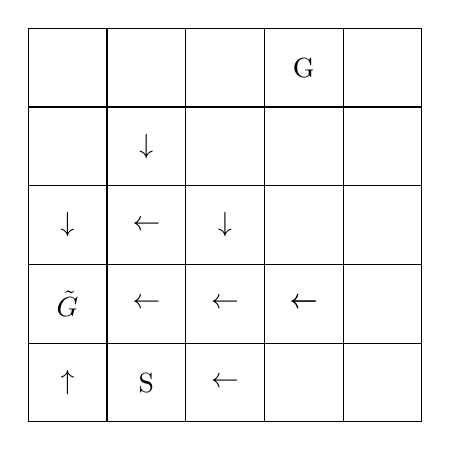
\begin{tikzpicture}
			\foreach \x in {0,1,2,3,4}{
				\foreach \y in {0,1,2,3,4}{
					\draw (\x,\y) rectangle +(1,1);
				}
			}
			\node at (0.5,1.5){\(\tilde{G}\)};
			\node at (1.5,1.5){\(\leftarrow\)};
			\node at (1.5,2.5){\(\leftarrow\)};
			\node at (2.5,1.5){\(\leftarrow\)};
			\node at (3.5,1.5){\(\leftarrow\)};
			\node at (2.5,0.5){\(\leftarrow\)};
			\node at (3.5,1.5){\(\leftarrow\)};
			\node at (0.5,2.5){\(\downarrow\)};
			\node at (1.5,3.5){\(\downarrow\)};
			\node at (2.5,2.5){\(\downarrow\)};
			\node at (0.5,0.5){\(\uparrow\)};
			\node at (1.5,0.5){S};
			\node at (3.5, 4.5){G};
		\end{tikzpicture}
	\end{centering}
\end{wrapfigure}

In case of the \(\vep\)-greedy policy, the occasional exploratory actions will only cause a one step deviation from the shortest path to this secondary goal, and the algorithm will use its knowledge about the surroundings to quickly walk back towards this goal using subsequent greedy actions. While finding the larger goal, requires multiple subsequent exploratory actions, leading away from the secondary goal. 

Boltzmann exploration does not perform much better, as the actions leading to the secondary goal will be assigned higher probability, so finding the larger goal still requires a chain of unlikely actions. 

And since estimating confidence intervals around \(Q\) values without samples, is not really possible, the performance of interval estimation depends on how it handles unknown states. If it uses Boltzmann exploration in the beginning, it will obviously struggle too. And setting high ranges for the initial interval estimations results in very similar behaviour to optimistic initialization of the \(Q\) values. As the algorithm would then explore until the entire state space is explored. 

Another example for this sparse reward setting are small negative rewards littered around the state space. Most games have this problem, where there is only one big reward for beating the level, but there are many possibilities to lose during the level. This can result in the agent deciding, that the optimal way to play is not to play, i.e. achieve the small goal of avoiding to lose.  

A naive fix to this problem would be to favour chains of exploratory actions (i.e. increase the likelihood of an exploratory action following another), or similar adjustments. An out-of-the-box solution is, to modify the existing rewards, artificially making them less sparse. 

\subsubsection{Curiosity-Driven Exploration}

Inspired by human curiosity, intrinsic rewards for actions which do not immediately result in extrinsic reinforcement were suggested. There are mostly two types of intrinsic motivation algorithms \parencite{pathakCuriosityDrivenExplorationSelfSupervised2017}. One rewards reaching ``novel'' states, encouraging the agent to stay in unexplored territory before walking back to known extrinsic rewards. Where ``novelty'' could be a constant minus the number of visits, or anything else one might come up with. 

In the second approach the agent builds a world model which tries to predict the next state \(x_{t+1}\) given state \(x_t\) and action \(a_t\). This world model would be a function approximation algorithm (e.g. an artificial neuronal net) which would be trained on the samples generated. Surprising this world model results in an additional reward for the reinforcement algorithm. This encourages the agent to take actions which it does not understand (i.e. which the world model does not predict). But in this basic form, the agent would get addicted to white noise, i.e. situations where the next state is completely unpredictable but also not necessarily meaningful.

\textcite{pathakCuriosityDrivenExplorationSelfSupervised2017}
recently came up with a modification to fix this problem. They argue that the unpredictability is due to the fact, that these unpredictable state changes are not influenced by the agents actions. 
So they suggest a filter \(\Phi\) for the state space, which maps the state to a smaller feature space, which only represents the influenceable state of the world. This feature map \(\Phi\) is attained by training a neuronal net.

This neuronal net consists of two copies of a neuronal net with input neurons \(x_t\) and \(x_{t+1}\) respectively, which have fewer output neurons. These two outputs \(\Phi(x_t)\) and \(\Phi(x_{t+1})\) are then fed into a common net which has \(\hat{a}_t\) as output. Similar to autoencoders (c.f. \ref{appx:autoencoder}) compressing information with a bottleneck, this neuronal net has to compress \(x_t\) and \(x_{t+1}\) to the middle layer \(\Phi(x_t)\) and \(\Phi(x_{t+1})\).

\def\layersep{2.5cm}
\begin{wrapfigure}{l}{7cm}
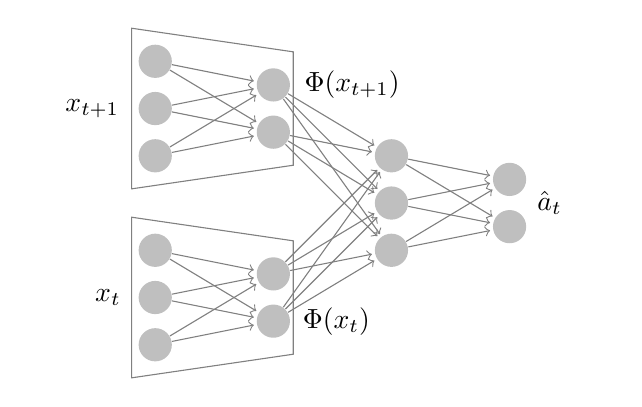
\begin{tikzpicture}[scale=0.6, shorten >=1pt,->,draw=black!50, node distance=\layersep]
    \tikzstyle{every pin edge}=[<-,shorten <=1pt]
    \tikzstyle{neuron}=[circle,fill=black!25,minimum size=12pt,inner sep=0pt]
    \tikzstyle{annot} = [text width=4em, text centered]

    % Draw the input layer nodes
    \foreach \name / \y in {1,...,3}
    % This is the same as writing \foreach \name / \y in {1/1,2/2,3/3,4/4}
        \node[neuron] (I-\name) at (0,4-\y) {};

    \node[annot, left of=I-2, node distance=0.8cm] {\(x_{t+1}\)};
    
    \foreach \name / \y in {4,...,6}
        \node[neuron] (I-\name) at (0,3-\y) {};

    \node[annot, left of=I-5, node distance=0.6cm] {\(x_{t}\)};

    % Draw the hidden layer 1 nodes
    \foreach \name / \y in {1,...,2}
        \node[neuron] (H1-\name) at (\layersep,3.5-\y) {};
    
    % Draw the hidden layer 1 nodes
    \foreach \name / \y in {3,...,4}
        \node[neuron] (H1-\name) at (\layersep,1.5-\y) {};

       
    % Draw the hidden layer 2 nodes
    \foreach \name / \y in {1,...,3}
        \node[neuron] (H2-\name) at (2*\layersep,2-\y) {};

    % Draw the output layer nodes
    \foreach \name / \y in {1,...,2}
        \node[neuron] (O-\name) at (3*\layersep,1.5-\y) {};

    % Connect every node in the input layer with every node in the
    % hidden layer 1.
    \foreach \source in {1,...,3}
        \foreach \dest in {1,...,2}
            \path (I-\source) edge (H1-\dest);

    % Connect every node in the input layer with every node in the
    % hidden layer 1.
    \foreach \source in {4,...,6}
        \foreach \dest in {3,...,4}
            \path (I-\source) edge (H1-\dest);
    
    % Connect every node in the hidden layer 1 with every node in the
    % hidden layer 2.
    \foreach \source in {1,...,4}
        \foreach \dest in {1,...,3}
            \path (H1-\source) edge (H2-\dest);
        
    % Connect every node in the hidden layer 3 with the output layer
    \foreach \source in {1,...,3}
        \foreach \dest in {1,...,2}
        \path (H2-\source) edge (O-\dest);

    % Annotate the layers
    \node[annot,right of=H1-1, node distance=1cm] {\(\Phi(x_{t+1})\)};
    \node[annot,right of=H1-4, node distance=0.8cm] {\(\Phi(x_t)\)};
    \node[annot] at (4*\layersep-47,0) {\(\hat{a}_{t}\)};

    \draw (-0.5,3.7) -- (\layersep+12, 3.2)--(\layersep+12, 0.8) --(-0.5,0.3)--cycle;
    \draw (-0.5,-3.7) -- (\layersep+12, -3.2)--(\layersep+12, -0.8) --(-0.5,-0.3)--cycle;
\end{tikzpicture}
\end{wrapfigure}
But since it does not need to recover the original from this compression but rather \(a_t\), it is meant to throw away the information about \(x_t\) which does not help to predict \(a_t\), i.e. throw away parts of the state space which can not be influenced by an action.

The world model then has to predict \(\Phi(x_{t+1})\) instead of \(x_{t+1}\), which means that its error will not increase when it does not predict non-influenceable changes like white noise, as these are filtered out by \(\Phi\).

This set-up proved extremely effective in empirical tests. It even learned to play some games, it was tested on, without any extrinsic reward at all. 

It might be argued, that this feature map \(\Phi\) filters out too many things, like actions by other actors which are not influenced by the agent itself, but influence the agent. If they influence the agent though, and the agent could, or should react to these actions, then these events will be relevant for predicting the agents actions. Therefore they would not be filtered out. Only if the agent can not, or has no incentive to respond to these events is it irrelevant for predicting the agents actions and will be filtered. And since the agent could not or does not need to react to these events anyway, no harm is done. 

\section{Function Approximation}

Up until now, we only discussed tabular methods, i.e. methods which store the value \(V(x)\) of a state \(x\) for every state in a table. There are two reasons for discarding this strategy. First, the state space might be simply too large to store \(V\) in that way (e.g. chess). Second, algorithms do not generalize at all with this method. If an algorithm ends up in a state where it never was before, the state can be almost identical to another state, and the algorithm will still treat it as completely unknown. If the input is a picture, it would be enough to change one pixel, one speck of dust and suddenly the algorithm treats the situation as completely new.

The solution is to use function approximation methods (i.e. supervised learning) to approximate the value functions. Function approximation tries to find the function from a reduced set of functions, which approximates the real function best. This reduced set of functions, might be the set of linear functions (linear regressions), the set of polynomials (polynomial regression), the trigonometric functions (Fourier analysis), the set of linear combinations of some universal kernel (support vector machines), the set of functions achievable with some weights in a neuronal net, or anything else one might come up with. There is usually some motivation for a particular set. Often the set, or a related superset, is dense in the set of continuous functions -- e.g. polynomials, trigonometric functions, the limits of linear combinations of universal kernels and linear combinations of sigmoid functions, which make up neuronal nets, are all dense in the set of continuous functions on some compact set.

Since the value function we are looking for will not be included in this reduced set of functions in general, we need to define some form of distance measure on the set of functions in order to pick the closest function in the reduced set. After that we can search for algorithms which converge to this closest function.

This more general setting of a reduced set of possible functions has two additional benefits:
\begin{enumerate}
	\item The reduced set of functions can exclude functions which can differentiate between hidden attributes of two states. Therefore this more general setting can model hidden information. 
	\item We can transform the limitation of memorylessness from a limitation of the MDP model to a limitation of the reduced (value) function set. I.e. we include the entire history in the state space, and force the reduced set of functions to only include value functions which depend on the last state only. Where the assumption, that the next state and reward depends only on the last state, was previously an assumption of the MDP, it now becomes an assumption of the function approximation. Function approximation with some form of memory, like recurrent neuronal nets with Long Short-Term Memory (LSTM), are then just a different reduced function set on the same MDP model.
\end{enumerate}
With these two observations, the underlying MDP becomes similar in kind, to the underlying sample space \(\Omega\) in probability theory. Whatever situation one might want to model, the MDP is large enough to perfectly model the situation by definition, and the restrictions are introduced later. In the case of probability theory by random variables, in the case of MDPs by the information available about the current state. This view tends to render all model based learning methods discussed in Section \ref{growing batch learning} useless, since it leaves the precise state, the agent is in, undefined, and the state space is too large to sample enough transitions in order to estimate transition probabilities anyway.

With this framework, video captured by a camera can be the observable part of the state, while everything that can not be observed by the camera is a hidden attribute of the state. But function approximation methods with memory can still achieve feats like object permanence, i.e. correctly assume objects still exists, after they have been covered up. 

There are also approaches which use unsupervised dimension reduction techniques on the inputs (principal component analysis, autoencoders, etc.), and use the resulting feature map as the state space. This allows for generalization, since multiple similar states are collapsed into one state. But it is also a special case of function approximation of the value function, since this is too just a restriction on the set of possible (value) functions. There are multiple reasons, why it might make sense to put such a dimension reduction module before the value function approximation:
\begin{enumerate}
	\item Consider the example of a robot using a camera to achieve a task. While letting the robot use its vision to try different behaviours takes real time of the robot moving around, training a dimension reduction algorithm on a bunch of pictures can be done without any real world interaction. Afterwards this pretrained function can be used in the value function approximation of the robot, speeding up the learning process. More generally:
	\begin{enumerate}
		\item data might already be available for some sub-task,
		\item some sub task might be cheaper to train on its own than the entire system,
		\item it might be easier to test reliability of subsystems, than getting enough data to verify the safety of the entire system (e.g. self-driving: a lot of data needed to verify the required safety improvement, since accidents are very rare)
	\end{enumerate}
	\item The ability to use model based learning techniques might be reintroduced by creating a state space using a feature map from a dimension reduction module (e.g. a deep autoencoder (c.f. \ref{appx:autoencoder}) in Deep Fitted Q Iteration \cite{langeBatchReinforcementLearning2012}). And even model free learning methods like experience replay can benefit from such a feature map, as it reduces the amount of memory need to store these experiences, and uncompressed video takes up an incredible amount of storage.
	\item Readers familiar with neuronal nets, might also be familiar with the vanishing/exploding gradient problem in deep neuronal nets with gradient decent. Pre-training lower layers promises to avoid this problem to some degree at least. 
\end{enumerate}

\subsection{Mean Squared Value Error}
As already noted, we require a distance measure on functions in order to determine the closest function in the reduced set. One such metric is 
\[
	d(f,g)\coloneqq\sum_{x\in\cX} \mu(x)[f(x)-g(x)]^2.
\]
where \(\mu\) is a probability measure on \(\cX\) weighting the states on how important they are. Let 
\(
	\{x\mapsto v(x,\mathbf{w})\}
\)
be the reduced set of functions with parameters \(\mathbf{w}\) (for example weights in a neuronal net). And \(v^*\) the objective function, then the \emph{mean squared value error} is defined as 
\[
	\widebar{\text{VE}}(\mathbf{w})\coloneqq d(v(\cdot,\mathbf{w}), v^*)
	= \sum_{x\in\cX} \mu(x)[v(x,\mathbf{w})-v^*(x)]^2.
\]
Now let \(X_0,X_1,\dots\) be a sequence in the state space, then we can often argue
\[
	\mu_n(x)=\mfrac{1}{n}\sum_{i=0}^{n-1} \mathbbm{1}_{x=X_i}\to \mu(x) \qquad (n\to \infty)
\]
for some probability measure \(\mu\). If the sequence \(X_0,X_1,\dots\) is generated with some behaviour \(\pi\) in an MDP for example, we can usually determine a limiting distribution. In order to avoid a degenerate limiting distribution in episodic MDPs, this generally requires a restart of the MDP whenever we reach a terminal state. This is useful, since it allows us to write
\[
	\mfrac{1}{n}\sum_{i=0}^{n-1}[v(X_i,\mathbf{w})-v^*(X_i)]^2 
	=\sum_{x\in\cX} \mu_n(x)[v(x,\mathbf{w})-v^*(x)]^2 \to \widebar{\text{VE}}(\mathbf{w}).
\]
And while the usefulness of this equation in gradient decent is most likely the main reason for using this particular \(\mu\), there is also a theoretical justification for it, since we care more about the accuracy of the value function on the states we actually visit than on states we do not visit anyway. 

\subsection{Very Short Introduction to Gradient Decent}

One heuristic to find the minimum of \(\widebar{\text{VE}}\), is to move in the direction of the steepest decent. This is in the opposite direction of the gradient:
\begin{align*}
	-\nabla \widebar{\text{VE}}(\mathbf{w})
	&= -\sum_{x\in\cX} \mu(x) \nabla[v(x,\mathbf{w})-v^*(x)]^2\\
	&=\lim_{n\to\infty} -\sum_{x\in\cX} \mu_n(x) \nabla[v(x,\mathbf{w})-v^*(x)]^2\\
	&=\lim_{n\to\infty} \nabla \mfrac{1}{n}\sum_{i=0}^{n-1}-[v(X_i,\mathbf{w})-v^*(X_i)]^2\\
	&= \lim_{n\to\infty} \mfrac{1}{n}\sum_{i=0}^{n-1} 2[v^*(X_i)-v(X_i,\mathbf{w})]\nabla v(X_i,\mathbf{w})
\end{align*}
But instead of making one step of size \(\tilde{\alpha}\) in this direction
\[
	\mathbf{w}_{t+1}
	=\mathbf{w}_t + \underbracket[0.7pt]{\tilde{\alpha}\mfrac{2}{n}}_{\eqqcolon \alpha} 
	\sum_{i=0}^{n-1} [v^*(X_i)-v(X_i,\mathbf{w}_t)]\nabla v(X_i,\mathbf{w}_t),
\]
we could also make \(n\) individual steps
\[
	\mathbf{w}_{t+1}
	=\mathbf{w}_t + \alpha [v^*(X_t)-v(X_t,\mathbf{w}_t)]\nabla v(X_t,\mathbf{w}_t).
\]
Since we update \(\mathbf{w}_t\) with every step, these two variants are not equivalent! But due to the higher frequency of updates in the second variant the hope is, that it converges more quickly. If we now just replace \(v^*(X_t)\) with \(U_t\) where \(\E[U_t\mid X_t]=v^*(X_t)\), and allow the learning rate to vary, then we obtain a regression 
\[
	\mathbf{w}_{t+1}
	=\mathbf{w}_t + \alpha_t [U_t-v(X_t,\mathbf{w}_t)]\nabla v(X_t,\mathbf{w}_t), 
\]
which is known as \emph{stochastic gradient decent} SGD. But note that the specifier ``stochastic'' refers to the selection of \(X_i\sim \mu\) and not \(U_t\). According to \textcite[202]{suttonReinforcementLearningIntroduction2018a} convergence proofs to a local minimum for SGD are available if the learning rate fulfils (\ref{learning rate conditions}). In particular this covers Monte Carlo with
\[
	U_t=\sum_{n=t}^\infty \gamma^{n-t} R_{n+1}.
\]
But since bootstrapping methods like TD and Q-learning, or more general n-step returns are not unbiased, these proofs are not applicable to them. Additionally the n-step return depends on the weights \(\mathbf{w}\):
\[
	\hat{V}^{(n)}(X_t,\mathbf{w})=R_{t+1}+\gamma R_{t+1}+ \dots +\gamma^{n-1}R_{t+n}+\gamma^n V(X_{t+n}, \mathbf{w})
\]
So this would have to be taken into account when differentiating with regard to \(\mathbf{w}\). But the regression
\[
	\mathbf{w}_{t+1}
	=\mathbf{w}_t + \alpha_t [\hat{V}^{(n)}(X_t,w_t)-v(X_t,\mathbf{w}_t)]\nabla v(X_t,\mathbf{w}_t),
\]
explicitly ignores this dependency and is thus grouped in \emph{semi-gradient methods} with other bootstrapping algorithms, that ignore this dependency.

\subsection{A counterexample}

There are certain interaction effects between bootstrapping methods and function approximation methods, which make the combination unstable. Consider the state space \(\cX=\{1,2\}\), let the action space \(\cA=\{1,2\}\) simply determine the next state (i.e. \(p(y\mid x,a)=\delta_{ya} \)), and imagine there are no rewards ever. Then consider the set of linear functions
\[
	\{v:x\mapsto w x :w\in\R\}.
\] 
In particular the true value function \(V^\pi=0\) (for all \(\pi\)) is included in the set. Now consider the transition from state \(X_0=1\) to state \(X_1=2\), when starting with some positive \(w_0\). Since there are no rewards, the update in TD(0) would be:
\begin{align*}
	w_1 
	&= w_0 + \alpha [0+\gamma v(X_1,w_0) - v(X_0,w_0)] \nabla v(X_0,w_0)\\
	&=w_0 + \alpha[\gamma 2w_0 - w_0] \cdot 1\\
	&=w_0 + \alpha \underbracket[0.7pt]{(2\gamma -1)}_{\ge 0 \mathrlap{\iff \gamma \le 1/2}} w_0
\end{align*}
So the value of \(w\) can actually increase! Even though it needs to move towards 0, since \(v(x,0)=V^\pi(x)\). It should be noted, that the valuation of the first state would increase in the tabular TD(0) version too, since the value of the state gets boosted by the fact, that it serves as an entryway to the higher valued state. But because of the interdependency of the evaluation of both states, the promise of this higher valued state causes the increase of the first state, which in turn increases the expectation for the value of the second state. So if we would just repeat the experience of a transition from state \(1\) to state \(2\), we would get into an ever increasing loop of expectations about the fantastic rewards that await us in state \(2\). But since TD(0) is actually on-policy, we will end up disappointed by the lack of rewards, when we actually reach state 2 and lower our expectations. 

But off-policy algorithms are not constrained by this requirement. Q-learning for example, evaluates the next state based on the optimal action possible in that state
\[
	\max_{b\in\cA_{X_{t+1}}}Q(X_{t+1}, b),
\]
with no consideration whether or not action \(b\) is actually enacted. Since the only off-policy algorithm I introduced was Q-learning, we need to adapt our example for action value functions. By modifying the available set of functions to
\[
	\{q: (x,a)\mapsto w a:w\in\R \},
\]
and assuming that the exploration policy always picks action \(1\), we always stay in the first state and thus end up with the iteration:
\begin{align*}
	w_{t+1} &=w_t+\alpha[0+\gamma 
	\overbracket[0.7pt]{\max_{b\in\cA_{X_{t+1}}}q(X_{t+1}, b,w_t)}^{
		=q(1,2,w_t)
	} - \overbracket[0.7pt]{q(X_t,A_t,w_t)}^{=q(1,1,w_t)}]
	\overbracket[0.7pt]{\nabla q(X_t,A_t,w_t)}^{=A_t=1}\\
	&=w_t + \alpha[ (2\gamma-1)w_t]> w_t \quad \iff \gamma>1/2 
\end{align*}
The exploration policy in this counter example is of course specially designed to cause divergence. This leads \textcite[263]{suttonReinforcementLearningIntroduction2018a} to hypothesize, that Q-learning might still be relatively stable for exploration policies, which are greedy enough, like \(\vep\)-greedy policies with small enough epsilon. They claim ``to the best of [their] knowledge, Q-learning has never been found to diverge in this case, but there has been no theoretical analysis''. 

Since it is the combination of function approximation, bootstrapping and off-policy learning, that causes such instability, \textcite[264]{suttonReinforcementLearningIntroduction2018a} dub this combination the ``deadly triad''. They claim that if any two elements are present, instability can be avoided. This claim is a bit of an oversimplification. \textcite{tsitsiklisAnalysisTemporaldifferenceLearning1997} present a proof, that TD(\(\lambda\)) with linear function approximation converges to some \(\mathbf{w}^\lambda\), which is not equal to the minimum\footnote{slight oversimplification since the minimum is not necessarily unique if the regressors are not linearly independent} \(\mathbf{w}^*\) in general, but can be bounded by:
\[
	d\left(v(\cdot,\mathbf{w}^\lambda), V^\pi\right)
	\le \frac{1-\lambda \gamma}{1-\gamma} \underbracket[0.7pt]{
		d(v(\cdot, \mathbf{w}^*), V^\pi)
	}_{
		=\min_{\mathbf{w}} \widebar{\text{VE}}(\textbf{w})
	}
\] 
So TD(\(\lambda\)) is stable enough to avoid divergence if \(\gamma<1\) (c.f. Subsection \ref{bootstrapping and discounting}) in the linear function approximation case, and its distance to the minimum in limit improves with \(\lambda\). And while this is far from perfect it appears to be a workable solution in practical applications. 

But for non linear function approximation \textcite{tsitsiklisAnalysisTemporaldifferenceLearning1997} also present an example, where TD(\(0\)) diverges. So it might simply be bootstrapping and function approximation which do not work well with each other. 

The reason for this incompatibility might be, that both concepts try to accomplish some sort of generalization. Temporal difference learning is supposed to generalize the existing estimates from older paths through the state space, to evaluations of new paths which cross states from older paths (c.f. Example \ref{driving home}). So these two methods have some overlap when it comes to their goals, which could explain why they get in each others way. But TD has no access to spatial similarity, which function approximation based on continuous functions automatically has, while function approximation does not have the theory of dynamic programming baked in. So neither method is a special case of the other.



%%%%%%%%%%%%%%%%%%%%%%%%%
\endinput
